\documentclass[11pt]{article}
\usepackage[UTF8]{ctex}
\usepackage{indentfirst}
%\setlength{\parindent}{2em}

% some package

% graph
\RequirePackage{graphicx}
\RequirePackage{subfigure}
\RequirePackage{float}
% math
\RequirePackage{amsmath}
\RequirePackage{amssymb,amsfonts,mathrsfs}

\RequirePackage{bm}         % \mathbf{}
\RequirePackage{color}      % the color of the font
\usepackage{mathrsfs}
\RequirePackage{enumerate}

% like word
\usepackage[top=2.54cm, bottom=2.54cm, left=3.17cm, right=3.17cm]{geometry}


%\usefonttheme{professionalfonts}

% the caption of thf figure
\renewcommand{\figurename}{图}


\title{ \textbf{贝叶斯网络} }


\author{
	邵逸岚  \qquad 21721121
}

\date{ }

\begin{document}
	
	\maketitle
	\section{定义}
		贝叶斯网络(Bayesian network)亦称信念网络(belief network),于1985年由Judea Pearl首先提出,是一种概率图模型,用来模拟人类推理过程中因果关系的不确定性处理模型。它借助有向无环图(Direct Acyclic Graph,简称DAG)来刻画属性之间的依赖关系,并使用条件概率表(Conditional Probability Table,简称CPT)来描述属性的联合概率分布。\par
		图1展示了一个简单的贝叶斯网络模型,a、b、c为属性,他们之间的有向边表示属性的依赖关系:\par
		\begin{figure}[htbp]
			\centering
			%\flushleft
			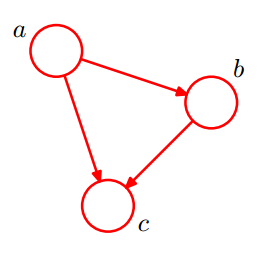
\includegraphics[width=0.4\textwidth]{img/simple_bn.png}
			\caption{简单贝叶斯网络}
			\label{001}
		\end{figure}
		一个贝叶斯网络B由结构G和参数$\Theta$两部分构成,即$B=\langle G,\Theta\rangle$。网络结构G是一个有向无环图,其中每个节点对应于一个属性,若两个属性有直接依赖关系,则它们由一条边连接起来;参数$\Theta$定量描述这种关系,假设属性$x_i$在G中的父节点集为$\pi_i$,则$\Theta$包含了每个属性的条件概率表$\theta_{x_i|\pi_i}=P_B(x_i|\pi_i)$。\par
		
	\section{结构}
		\subsection{基本结构}
			复杂的贝叶斯网络一般都可以分解为图\ref{0-002}的三种典型的依赖关系:\par
			\begin{figure}
				\centering
				\begin{tabular}{ccc}
					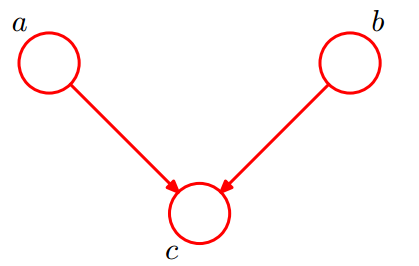
\includegraphics[width=0.28\linewidth]{img/head2head.png} &
					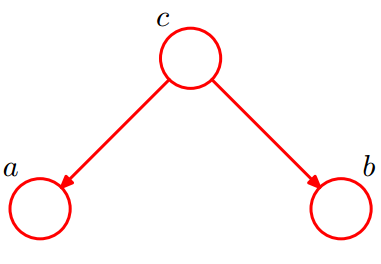
\includegraphics[width=0.28\linewidth]{img/tail2tail.png} &
					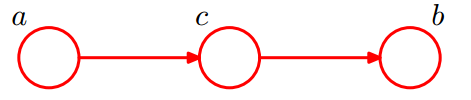
\includegraphics[width=0.28\linewidth]{img/head2tail.png}\\
					(a) & (b) & (c) \\
					~\\
				\end{tabular}
				\caption{贝叶斯网络中属性的典型依赖关系}
				\label{0-002}
				\vspace{-0.5em}
			\end{figure}
			(a)为head-to-head(V型)结构,在c未知的条件下,a、b被阻断(blocked),是独立的:
			$$\sum_{c}P(a,b,c)=\sum_{c}P(a)P(b)P(c|a,b)\Rightarrow P(a,b)=P(a)P(b)$$\par
			(b)为tail-to-tail(同父)结构,在c给定的条件下,a,b被阻断(blocked),是独立的:
			$$P(a,b,c)=P(c)P(a|c)P(b|c)\Rightarrow P(a,b|c)=P(a|c)P(b|c)$$\par
			(c)为head-to-tail(顺序)结构,在c给定的条件下,a,b被阻断(blocked),是独立的:
			$$P(a,b|c)=\frac{P(a,b,c)}{P(c)}=\frac{P(a,c)P(b|c)}{P(c)}=P(a|c)P(b|c)$$\par
			
		\subsection{联合概率分布}
			贝叶斯网络结构有效地表达了属性间的条件独立性。给定父节点集,贝叶斯网络假设每个属性与它的非后裔属性独立,于是$B=\langle G,\Theta\rangle$将属性$x_1, x_2, ..., x_d$的联合概率分布定义为:\par
			$$P_B(x_1,x_2,...,x_d)=\prod_{i=1}^{d}P_B(x_i|\pi_i)=\prod_{i=1}^{d}\theta_{x_i|\pi_i}$$
			以图\ref{001}为例,联合概率分布定义为:\par
			$$P(a,b,c)=P(a)P(b|a)P(c|a,b)$$
		
	\section{特点}
		贝叶斯网络的训练比较复杂,是一个NP-complete问题,也就是说,现阶段没有可以在多项式时间内完成的算法。但是对于某些应用,这个训练过程可以简化,并在计算上高效实现。\par
		它本身是一种不定性因果关联模型,是将多元知识图解可视化的一种概率知识表达与推理模型,更为贴切地蕴含了网络节点变量之间的因果关系及条件相关关系。贝叶斯网络具有强大的不确定性问题处理能力。贝叶斯网络用条件概率表达各个信息要素之间的相关关系,能在有限的、不完整的、不确定的信息条件下进行学习和推理。\par
		贝叶斯网络能有效地进行多源信息表达与融合。贝叶斯网络可将故障诊断与维修决策相关的各种信息纳入网络结构中,按节点的方式统一进行处理,能有效地按信息的相关关系进行融合。
	
	\section{应用}
		贝叶斯网络可以用来表达错综复杂的相互关系,最初主要用于处理人工智能中的不确定性信息。随后它逐步成为了处理不确定性信息技术的主流,并且在计算机智能科学、工业控制、医疗诊断等领域的许多智能化系统中得到了重要的应用。\par
		下图为贝叶斯网络在医疗诊断上的应用:\par
		\begin{figure}[htbp]
			\centering
			%\flushleft
			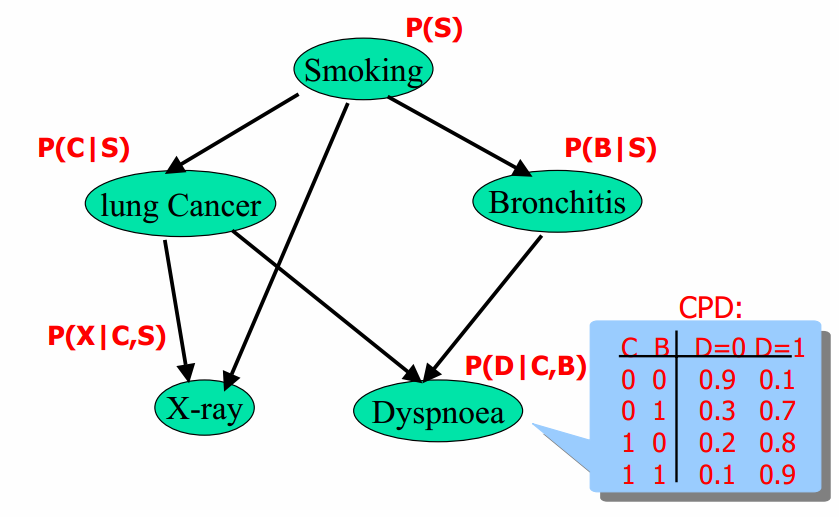
\includegraphics[width=0.7\textwidth]{img/instance.png}
			\caption{贝叶斯网络实例}
			\label{003}
		\end{figure}
		Smoking表示吸烟,其概率用$P(S)$表示,lung Cancer表示的肺癌,一个人在吸烟的情况下得肺癌的概率用$P(C|S)$表示,X-ray表示需要照医学上的X光,肺癌可能会导致需要照X光,吸烟也有可能会导致需要照X光(所以smoking也是X-ray的一个原因),因吸烟且得肺癌而需要照X光的概率用$P(X|C,S)$表示。Bronchitis表示支气管炎,一个人在吸烟的情况下得支气管炎的概率用$P(B|S)$,dyspnoea表示呼吸困难,支气管炎可能会导致呼吸困难,肺癌也有可能会导致呼吸困难(所以lung Cancer也是dyspnoea的一个原因),因吸烟且得了支气管炎导致呼吸困难的概率用$P(D|C,B)$表示。\par
		我们根据贝叶斯网络,由一个人的临床症状大概可以推断出他罹患肺癌和支气管炎的概率,由一个人的患病情况也可以推断出这个人是否由吸烟的习惯等等。
	
	\section{总结}
		贝叶斯理论是处理不确定性信息的重要工具,是常见的复杂网络之一。作为一种基于概率的不确定性推理方法,贝叶斯网络在处理不确定信息的智能化系统中已得到了重要的应用,已成功地用于医疗诊断、统计决策、专家系统、学习预测等领域。这些成功的应用,充分体现了贝叶斯网络技术是一种强有力的不确定性推理方法。
			
	
% bibe
\bibliographystyle{plain}
\end{document}


